\documentclass[12pt]{article}
\usepackage[paper=letterpaper,margin=2cm]{geometry}
\usepackage{amsmath}
\usepackage{amssymb}
\usepackage{amsfonts}
\usepackage{newtxtext, newtxmath}
\usepackage{enumitem}
\usepackage{titling}
\usepackage[colorlinks=true]{hyperref}
\usepackage{graphicx}
\usepackage{csvsimple}
\usepackage{luacode}
\setlength{\droptitle}{-6em}

% Enter the specific assignment number and topic of that assignment below, and replace "Your Name" with your actual name.

\title{\textbf{COMP0086 Summative Assignment}}
\author{Student Numbers: 21168615 \& 19004608 \\ }
\date{Nov 16, 2022}

\begin{document}
    \maketitle
\begin{enumerate}[leftmargin=\labelsep]
\section{PART I}
\subsection{Linear Regression}
\item[1.]
    \begin{enumerate}
        \item Superimposing the four different curves corresponding to each fit over the four given data points:
        \begin{figure}[h!]
        \centering
        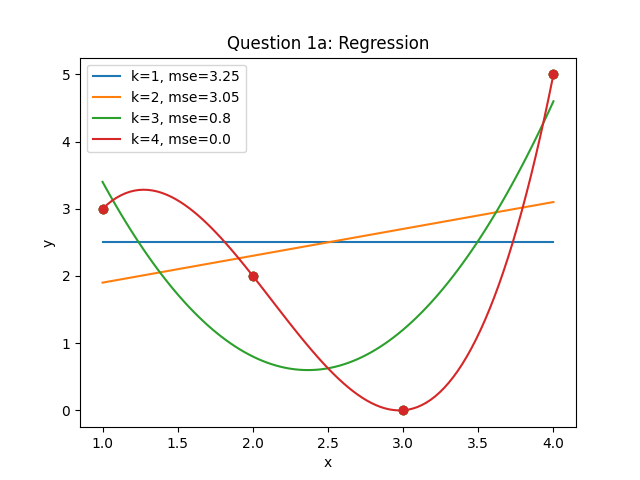
\includegraphics[scale=0.5]{outputs/q1/q1a}
        \caption{Data set $\{(1, 3), (2, 2), (3, 0), (4, 5)\}$ fitted with basis $\{1, x\}$ and basis $\{1, x, x^2, x^3\}$ }
        \label{fig:1a}
        \end{figure}

        \item The weights for the equations:
        \begin{center}
        \begin{tabular}{c|c|c|c|c}%
         \textbf{Basis}&\textbf{k=1}&\textbf{k=2}&\textbf{k=3} &\textbf{k=4}% specify table head
        \csvreader[head to column names]{outputs/q1/q1b.csv}{}% use head of csv as column names
        {\\\hline\csvcoli&\csvcolii&\csvcoliii&\csvcoliv&\csvcolv}% specify your coloumns here
        \end{tabular}
        \end{center}

        \item The mean squared error for each fitted curve:
        \begin{center}
        \begin{tabular}{c|c|c|c|c}%
         \textbf{Metric}&\textbf{k=1}&\textbf{k=2}&\textbf{k=3} &\textbf{k=4}% specify table head
        \csvreader[head to column names]{outputs/q1/q1c.csv}{}% use head of csv as column names
        {\\\hline\csvcoli&\csvcolii&\csvcoliii&\csvcoliv&\csvcolv}% specify your coloumns here
        \end{tabular}
        \end{center}
    \end{enumerate}
\newpage
\item[2.]
    \begin{enumerate}
        \item
        \begin{enumerate}
            \item Plotting the function $sin^2(2\pi x)$ in the range $0 \leq x \leq 1$ with the sampled points superimposed:
                    \begin{figure}[h]
                    \centering
                    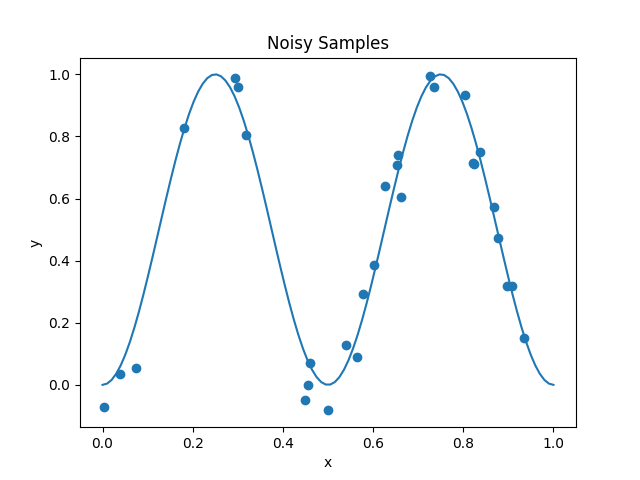
\includegraphics[scale=0.5]{outputs/q2/q2ai}
                    \caption{Noisy samples}
                    \label{fig:2ai}
                    \end{figure}
            \item Fitting the data set with polynomial bases of dimension $k = 2, 5, 10, 14, 18$ and plotting each of these 5 curves with the sampled points superimposed:
                    \begin{figure}[h]
                    \centering
                    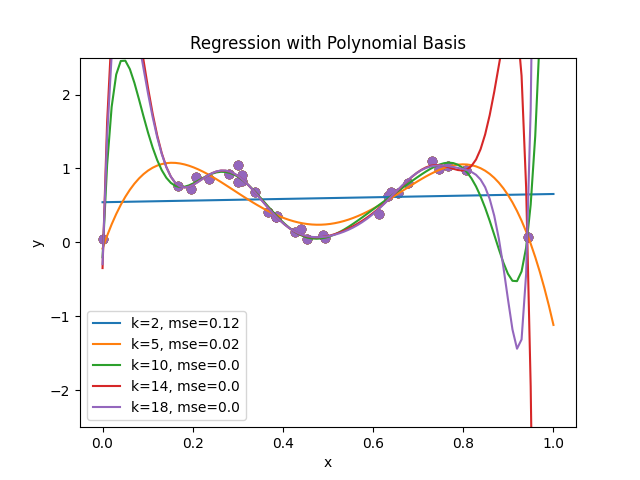
\includegraphics[scale=0.5]{outputs/q2/q2aii}
                    \caption{Polynomial fit curves}
                    \label{fig:2aii}
                    \end{figure}
        \end{enumerate}
\newpage
        \item[(b \& c)] Plotting the $\ln$ of the train and test error for a single trial of 1000 test points versus the polynomial dimension $k = 1, . . . , 18$:
            \begin{figure}[h]
            \centering
            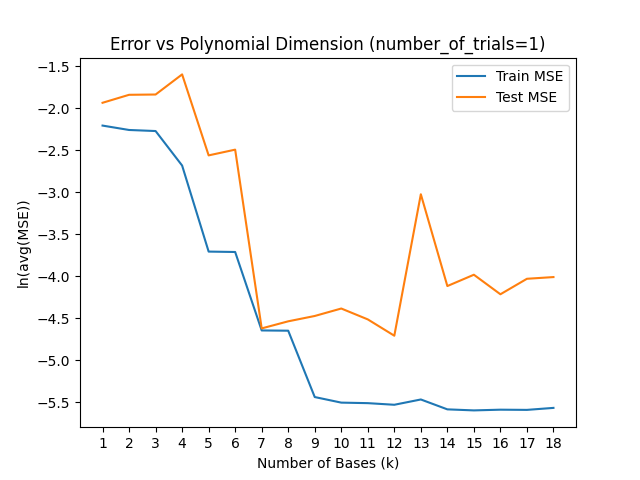
\includegraphics[scale=0.5]{outputs/q2/q2bc}
            \caption{Training and Testing Error of Polynomial Curves (1 trial)}
            \label{fig:2c}
            \end{figure}
        \item[(d)] Plotting the $\ln$ of the train and test error for 100 trials of 1000 test points versus the polynomial dimension $k = 1, . . . , 18$:
            \begin{figure}[h]
            \centering
            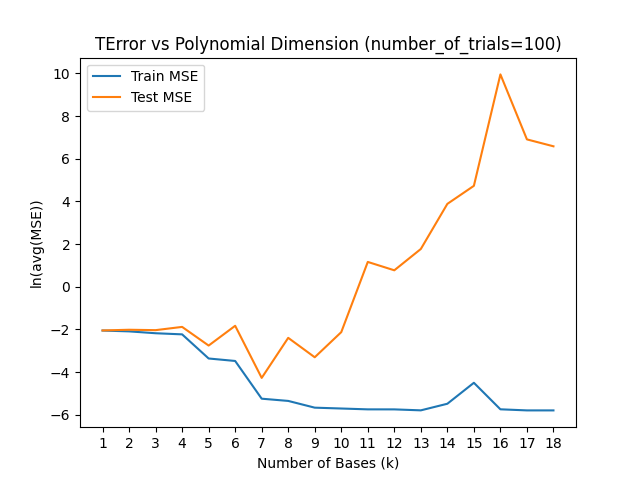
\includegraphics[scale=0.5]{outputs/q2/q2d}
            \caption{Training and Testing Error of Polynomial Curves (100 trials)}
            \label{fig:2d}
            \end{figure}
    \end{enumerate}
\newpage
\item[3.] Repeating 2 (b-d) with $\sin$ basis functions:
            \begin{figure}[h]
            \centering
            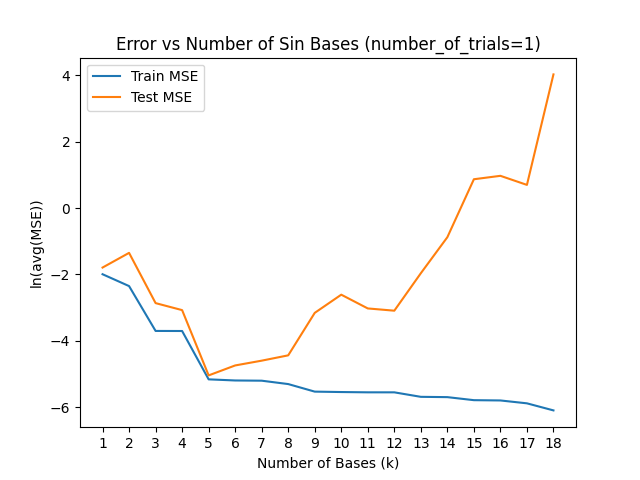
\includegraphics[scale=0.5]{outputs/q3/q3bc}
            \caption{Training and Testing Error of $\sin$ Curves}
            \label{fig:3b}
            \end{figure}
            \begin{figure}[h]
            \centering
            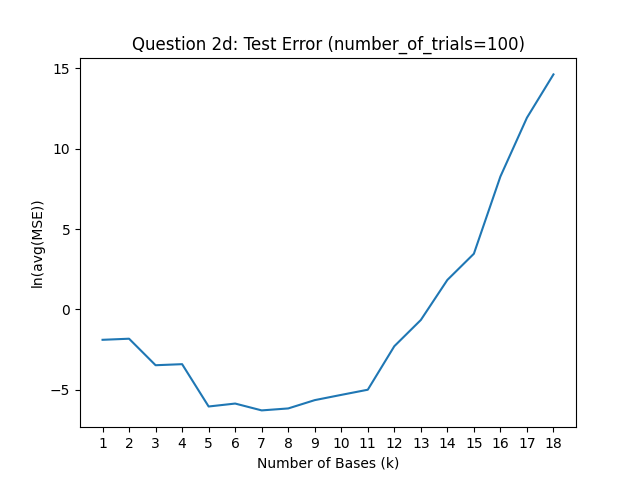
\includegraphics[scale=0.5]{outputs/q3/q3d}
            \caption{Testing and Testing Error of $\sin$ Curves (100 trials)}
            \label{fig:3d}
            \end{figure}
\newpage
\subsection{Filtered Boston housing and kernels}
    \item[4.]
    \begin{enumerate}
        \item[(b)]
        We interpret the naive linear regression model using the existing framework for least squares regressors.\\
        Namely, we have:\\
        $w^* = (X^TX)^{-1}X^{T} y, X = (1,\dots,1)^{T} $\\
        \[\implies w* = m^{-1}  \sum_{i} 1*y_{i} = \bar{y}\]\\
        \[\implies f(x_{i}) = 1 \times w^{*} = \bar{y}\]\\
        Our model in this case is essentially always predicting the average housing price in the training data set.
%        We split the data using our train test split function, and train naive, single and multiple linear regression models.
%            We repeat this 20 times and report the MSE on training and test sets.\\

        \item[(a,c,d)] Here is a table of the training and test mean squared errors:\\
        \begin{center}
        \scalebox{0.8} {\begin{tabular}{c|c|c|c|c}%
         \textbf{Model}&\textbf{Train Mean}&\textbf{Train St. Dev.}&\textbf{Test Mean} &\textbf{Test St. Dev.}% specify table head
        \csvreader[head to column names]{outputs/q4/performance.csv}{}% use head of csv as column names
        {\\\hline\csvcoli&\csvcolii&\csvcoliii&\csvcoliv&\csvcolv}% specify your coloumns here
        \end{tabular}
        }
        \end{center}
    \end{enumerate}
\newpage
\subsection{Kernelised ridge regression}
\item[5.]
%We fit our kernel ridge regressors for each parameter pair over 5 cross validation folds,
%and search for the pair minimising our mean squared error.\\

%Here are the optimal parameters along with the minimal mean squared error:\\


%The mean squared error for each fitted curve:
%\begin{center}
%\begin{tabular}{c|c|c}%
%\textbf{Gamma}&\textbf{Sigma}&\textbf{MSE}% specify table head
%\csvreader[head to column names]{outputs/q5/optimal_gkrr_parameters.csv}{}% use head of csv as column names
%{\\\hline\csvcoli&\csvcolii&\csvcoliii}% specify your coloumns here
%\end{tabular}
%\end{center}
%
%\\

    \begin{enumerate}
\item[(a)] The optimal parameters:

    \begin{center}
    \scalebox{0.8} {\begin{tabular}{c|c|c|c|c}%
     \textbf{Trial}&$\log_2(\sigma)$&$\log_2(\gamma)$ % specify table head
    \csvreader[head to column names]{outputs/q5/q5a-optimal-params.csv}{}% use head of csv as column names
    {\\\hline\csvcolii&\csvcoliii&\csvcoliv}% specify your coloumns here
    \end{tabular}
    }
    \end{center}

\item[(b)] Displaying the logarithm of the mean 5 fold mean squared error for different parameters for a single trial:\\

\begin{centering}
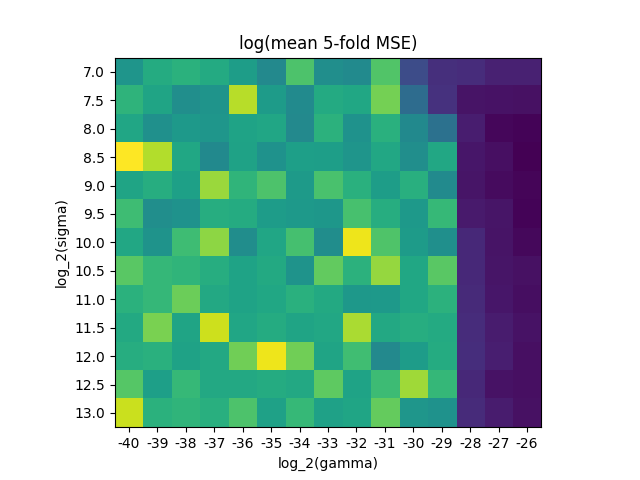
\includegraphics[scale = 0.5]{outputs/q5/q5b-cross-valid-error}\\
\end{centering}
\item[(c)]The mean squared error for the training and test sets for the best $\gamma$ and $\sigma$ for a single trial:
    \begin{center}
    \scalebox{0.8} {\begin{tabular}{c|c|c|c|c}%
     \textbf{Model}&\textbf{Train Mean}&\textbf{Test Mean} % specify table head
    \csvreader[head to column names]{outputs/q5/q5c-performance.csv}{}% use head of csv as column names
    {\\\hline\csvcoli&\csvcolii&\csvcoliv}% specify your coloumns here
    \end{tabular}
    }
    \end{center}



\item[(d)]The mean squared error for each fitted curve over 20 runs:
        \begin{center}
        \scalebox{0.8} {\begin{tabular}{c|c|c|c|c}%
         \textbf{Model}&\textbf{Train Mean}&\textbf{Train St. Dev.}&\textbf{Test Mean} &\textbf{Test St. Dev.}% specify table head
        \csvreader[head to column names]{outputs/q5/q5d-performance.csv}{}% use head of csv as column names
        {\\\hline\csvcoli&\csvcolii&\csvcoliii&\csvcoliv&\csvcolv}% specify your coloumns here
        \end{tabular}
        }
        \end{center}
    \end{enumerate}
\newpage
\section{PART II}
\subsection{$k$-Nearest Neighbors}
\item[6.]Generating a random $h$:
            \begin{figure}[h]
            \centering
            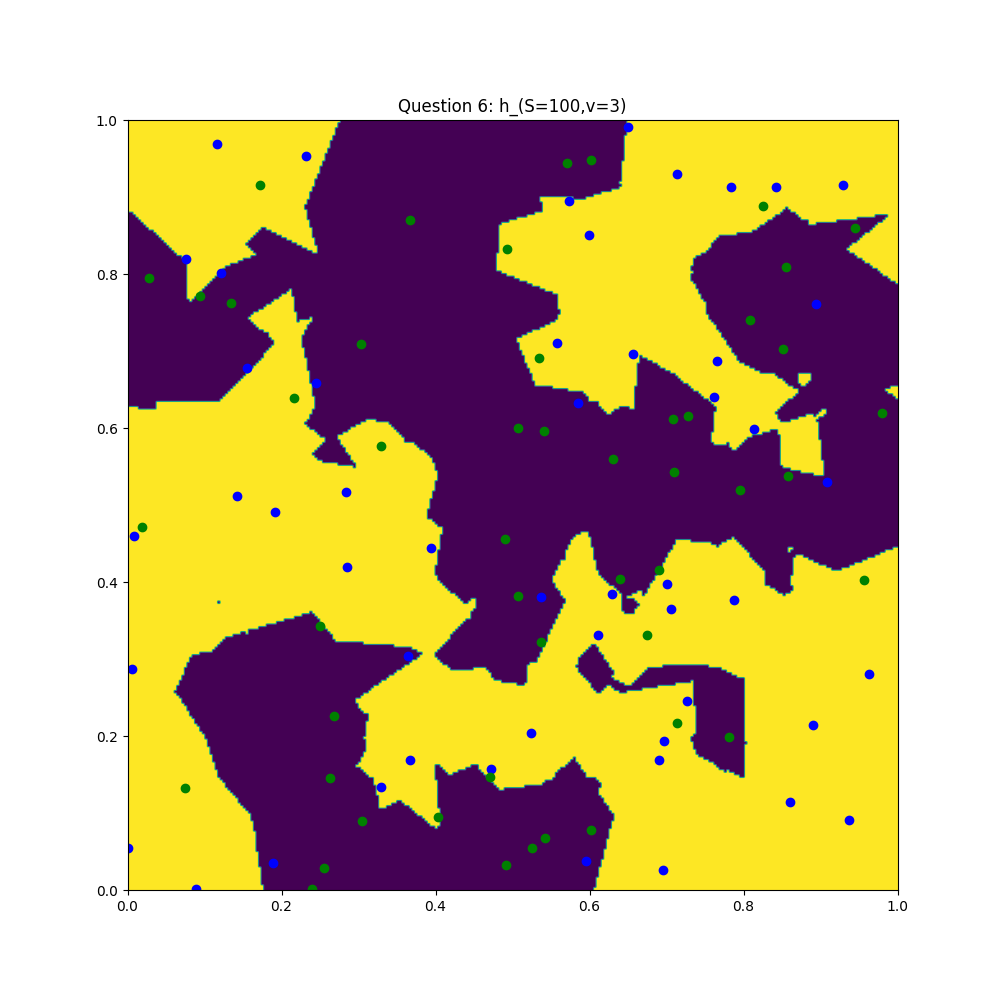
\includegraphics[scale=0.5]{outputs/q6/q6}
            \caption{A hypothesis $h_{S,v}$ visualised with $|S|=100$ and $v=3$}
            \label{fig:6a}
            \end{figure}
\newpage
\item[7.]
    \begin{enumerate}
        \item Producing a visualisation using Protocol A:
            \begin{figure}[h]
            \centering
            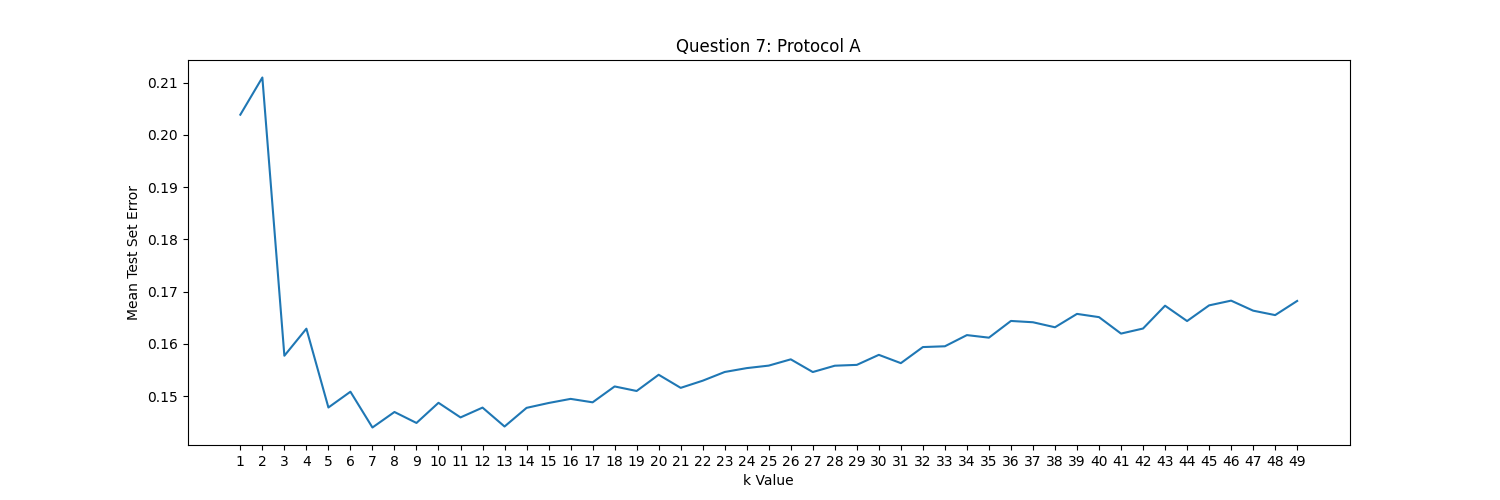
\includegraphics[scale=0.5]{outputs/q7/q7}
            \caption{Protocol A}
            \label{fig:7}
            \end{figure}
        \item We know that the data generating process uses $v=3$, so we would have initially expected the smallest test error to be located at the matching k-value, $k=3$.
        However, the data generating process for the training data set labels \textit{and} the testing data set labels were injected with noise, so k-values greater than 3 have a ``de-noising'' effect allowing for better performance at around $k=7$.
        As the k-value increases beyond $k=7$, this smoothing effect is too strong, causing the gradual increase in test error as the k value increases.
        For $k<7$ and in particular $k<v=3$ we see the error growing because the model has small $k$ and is able to fit to the noise injected into the data generating process, corrupting the model.
        By averaging over 100 runs, the plot is relatively smooth allowing us to make generalisations about the relationship between k-value and mean test set error.
    \end{enumerate}
\newpage
\item[8.]
    \begin{enumerate}
        \item Producing a visualisation using Protocol B:
            \begin{figure}[h]
            \centering
            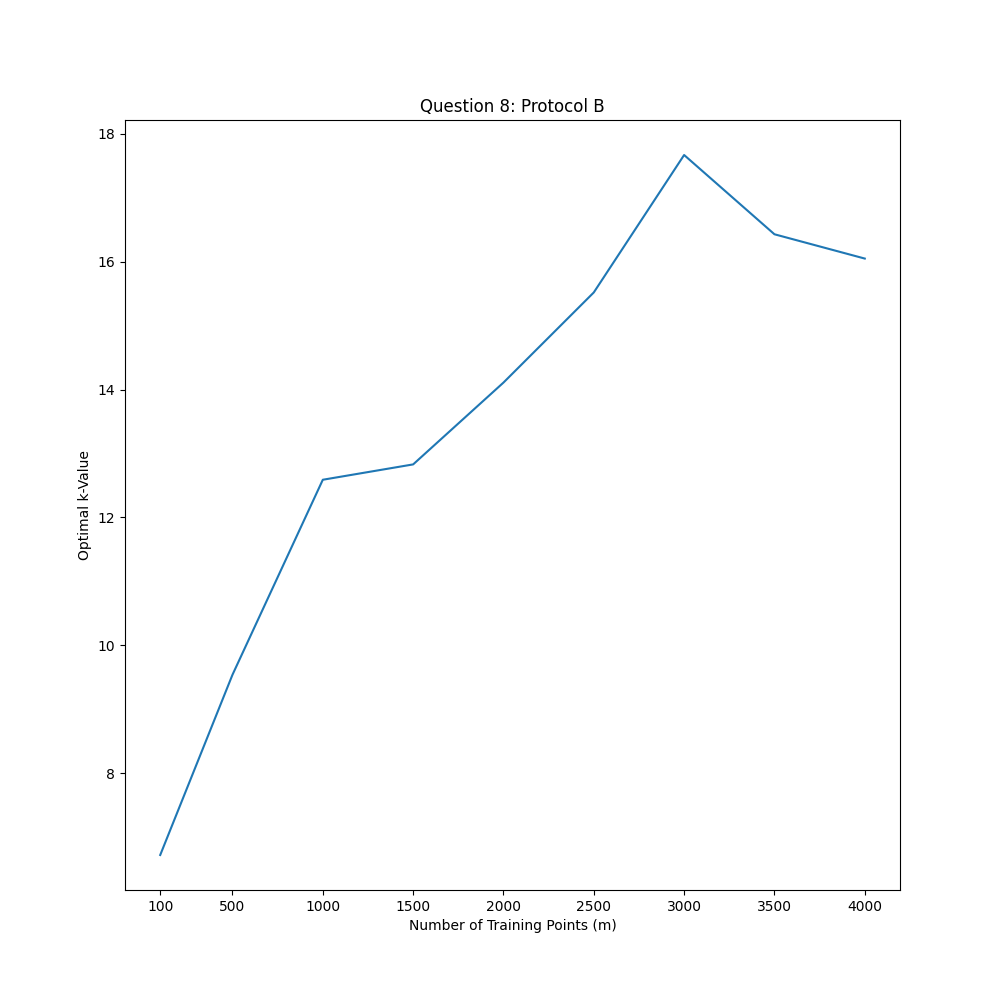
\includegraphics[scale=0.5]{outputs/q8/q8}
            \caption{Protocol B}
            \label{fig:8}
            \end{figure}
        \item k-nearest neighbours is a non-parametric model, so when queried with a test point for prediction, the number of training points within a given fixed radius of that test point increases as the number of training points increases.
        If we consider this fixed radius `sufficiently close' to make an informed prediction, the number of points within this radius will increase with more training points.
        So as the number of training points increases, the optimal k would increase to include more of the training points within this same fixed radius.
        We can see in the plot above that we see this general trend as expected, however there is some noise in the trend and so a smoother plot would likely requires more runs.
    \end{enumerate}
\newpage
\section{PART III}
\subsection{Questions}
\item[9.] \begin{enumerate}
              \item let $K_{c}(\textbf{x},\textbf{z}) = c+ \sum_{i=1}^{n}x_{i}z_{i} = c + \textbf{x}^{T}\textbf{z}$\\
        Our function $K_{c}(\cdot, \cdot)$ is psd iff:\\
        $\forall \{ u_{i} \}_{1:m} \in \mathcal{R}, {\{\textbf{x}_{j}\}_{1:m} \in \mathcal{R}^{n}$:

        $\sum_{k,l} u_{k}u_{l}K_{c}(\textbf{x}_{k},\textbf{x}_{l}) \ge 0 $\\
        We expand our kernel function to give: \\
        \[\sum_{k,l} u_{k}u_{l}K_{c}(\textbf{x}_{k},\textbf{x}_{l}) =  \sum_{n,m} cu_{n} u_{m} + \sum_{n,m} \langle\textbf{x}_{n}, \textbf{x}_{m}\rangle u_{n} u_{m}\]

        Here, we note that $\langle \cdot, \cdot \rangle$ is an inner product over the Hilbert space $\mathcal{R}^{n}$ and hence is psd by the representer theorem:
                \begin{equation}
        \implies \sum_{n,m} \langle\textbf{x}_{n},
        \textbf{x}_{m}\rangle u_{n} u_{m} \ge 0
                \end{equation}

        \textbf{Proposition}
        $K_{c}(\cdot, \cdot)$ is psd iff $c \ge0$ \\
        \textbf{Proof:}\\
        $(\implies)$\\

        Suppose $c \ge 0$.

         $(1) \implies \sum_{k,l} u_{k}u_{l}K_{c}(\textbf{x}_{u},\textbf{x}_{l}) \ge c \sum_{n,m}u_{n}u_{m} = c (\sum_{n}u_{n})^{2} \ge 0$\\

        $(\impliedby)$\\

        let $c < 0$.
        Suppose our vectors $x_{n}$ are identically equal to $ (\sqrt{a},0)^{T}$, for some $a < |c|/n \implies x_{k}^{T}x_{l} = a $\\
        $\forall k,l$.\\

        $\implies \sum_{k,l} u_{k}u_{l}K_{c}(\textbf{x}_{u},\textbf{x}_{l}) = (a+c) \sum_{n,m}u_{n}u_{m} = (a + c)(\sum_{n}u_{n})^{2} < 0$\\
        Hence for any $c < 0$, $
        \exists \{ u_{i} \}_{1:m} \in \mathcal{R},
         \{ \textbf{x}_{j}\}_{1:m} \in \mathcal{R}^{n}$s.t:\\
           $\sum_{k,l} u_{k}u_{l}K_{c}(\textbf{x}_{u},\textbf{x}_{l}) < 0
        \square$
    \item Using this kernel in our ridge regression, we note that as the value of c increases, the value of the kernel converges to a single value, c. More concretely, the 
    kernel between any 2 datapoints becomes relatively uniform. We may infer from this that adding a constant in our kernel function has a regularising effect, as the model.\\
    Expanding on this we demonstrate that we converge to naive linear regression in the limit:\\

    Note as $c \to \infty$, $K  = XX^T + c 1_{nxn} \to c 1_{nxn} = c 1_{n} 1_{n}^T$, where $1_{l,m}$ is an lxm dimensional vector a=of all ones. Note the similarity here with naive linear regression, where $X =1_{n}$.\\
    
    $\alpha = c^{-1} $leastsquares$(1_{nxn}, y_{train})$ (we no longer assume invertibility)\\
    $\implies \hat{y}_{test} = c \alpha 1_{n_{train},n_{test}} = 1_{n_{train},n_{test}} $leastsquares$(1_{nxn}, y_{train})$\\

     Hence for our predictions, the constants c cancel out and we are left with the exact dual form of naive linear regression:\\
     
     $\alpha \prime = leastsquares$(1_{nxn}, y_{train}) = \overline{y}_{train}$\\
     $y_{test} = \alpha \prime 1_{n_{train},n_{test}} = [\overline{y}_{train}]_{1:n_{train}}$
    Hence,
    Hence, adding c to our kernel acts like a regulariser.\\ 
\end{enumerate}

\newpage
\item[10.]  Define $g(t) := $sgn$(f(t)) = \frac{f(t)}{| f(t)|}$\\
    \textbf{Proposition:}\\
    
    as $\beta \to \infty$, $g(t) \to 1-NN$\\
    
    \textbf{Proof:}\\
    
    $f(t) = \sum_{i} \alpha_{i} K(x_{i}, t)$, where $ \alpha = (K + \gamma I_{l})^{-1} y$\\
    
    since $K(x,x) = exp(0) = 1$ for  all x, we decompose K as follows:\\
    
    $K = I_{l} + \tilde{K}$, where $\tilde{K}_{ij} = K(x_i, x_j)$, $i \ne j$. We note here that as $\beta \to \infty$, $\tilde{K} \to 0$.\\
    
    We take a taylor expansion in $\tilde{K}$, to arrive at the following result:\\

    $\alpha = ((\gamma+1) I_{l} + \tilde{K})^{-1} y = \frac{1}{\gamma + 1} (I_{l} - O(\tilde{K})) y $
    Hence as $\beta \to \infty$, $\alpha \to \frac{1}{\gamma +1}y$\\
    Hence our predictor function becomes:\\
    $f(t) \to \frac{1}{\gamma+1} \sum_{i} y_{i} K(x_{i}, t) \implies g(t)  \to \frac{\sum_{i} y_{i} K(x_{i}, t)}{|\sum_{i} y_{i} K(x_{i}, t)|}
    $\\

    Let's assume that there exists a unique point x in our training set of minimal distance to our test point.\\
    Define $d_{i} := \|x_{test} - x_{i}\|^{2}$, and $d* := min_{i} d_{i}$\\
    $g(t) = \frac{y_{*} exp(-\beta d_{*})}{|\sum_{i} y_{i} exp(-\beta d_{i})|} + \sum_{i\ne *}\frac{y_{i} exp(-\beta d_{i})}{|\sum_{i} y_{i} exp(-\beta 
    d_{i})|} = \frac{y_{*}}{|y_{*} + \sum_{i \ne *} y_{i} exp(-\beta (d_{i} - d_{*}))|} + \sum_{i\ne *}\frac{y_{i} exp(-\beta (d_{i} - d_{*}))}{|y_{*} + \sum_{i \ne *} y_{i} exp(-\beta (d_{i} - d_{*}))|}$.\\
    
    Note for $d_{i} \ne d_{*}$, $exp(-\beta(d_{i} - d_{*})) \to 0$ as $\beta \to \infty$. Hence:\\
    $g(t) \to \frac{y_{*}}{|y_{*} + 0|} + \frac{0}{|y_{*} + 0|} = y_{*} = y_{i} : x_{i} = min_{i} \|x_{test} - x_{i}\|$ which is the required 1-NN predictor.\\
    
\newpage
\item[11.] \\
Given a whack-a-mole grid of size n, it is solvable if we can apply a sequence from our $n^{2}$ permissible moves that results in a blank screen. We first index all permissible moves by $T_{i,j}$, which has the effect of flipping the state of squares $(i,j),(i-1,j),(i+1,j),(i,j-1)(i,j+1)$, as long as each coordinate is still on the grid.\\
We may consider each grid as an element of the space of square matrices over $\mathcal{F}_{2}$, the finite field of order 2: under this construction, we see that the application of a move $T_{i,j}$ corresponds to the sum between the grid and a matrix $T_{ij}$, where $T_{ij}$, where the entries of $T_{ij}$ are zero everywhere except at $(i,j),(i-1,j),(i+1,j),(i,j-1)(i,j+1)$, if these values are present on the grid. For example, if n = 4, the transformation $T_{2,2}$ corresponds to the addition of the matrix $T_{22}$:\\
    
   $T_{22} = $ \begin{pmatrix}
    0 & 1 & 0 & 0\\
    1 & 1 & 1 & 0\\
    0 & 1 & 0 & 0\\
    0 & 0 & 0 & 0\\
    \end{pmatrix}
    \\
    Since our operations on a grid are now simply the sum of matrices over a $\mathcal{F}_{2}$, it is now immediately obvious that our operations are commutative, by the commutativity of addition.\\
    Further, since applying the same operation twice would be the same as applying the matrix twice in order, we can see that any operation applied twice would have the effect of applying no operation at all ( since $T_{ij} + T_{ij} = 0)$.\\
    Hence, we conclude for $1 \le i,j \le n$, each operation is applied at most once. From this point, we note that there is no reason for our operations to be square matrices, as the only required properties of the space are those of a vector space (we make no use here of matrix multiplication). Hence, we may vectorise both our input grid and our operation matrices to get a set of vectors over $\mathcal{F}_{2}^{n^2}$. We now index our operation vectors $t_i: i = 1, \dots, n^2$.\\
    Let $x_{i} = \mathcal{I} [t_{i} $ is used $]$ be an indicator function representing whether $t_i$ is added to the input to get our blank grid.\\
    We observe that our problem is solvable for a given input grid G (now vectorised as a vector \textbf{g}) iff there exists a vector \textbf{x} $\in \mathrm{F}_{2}^{n^2}$ st:\\
    $\sum_{i} t_{i} x_{i} + \mathbf{g} = \mathbf{0}.$\\
    If we stack the vectors $t_{i}$ horizontally as the columns of a matrix T, we get:\\
    $T\mathbf{x} + \mathbf{g} = 0$\\
    Since every element is its own additive inverse over $\mathcal{F}_{2}$, we add $\mathbf{g}$ to both sides and arrive at the linear system $T \mathbf{x} = \mathbf{g}$.\\
    Since the matrix T may not be invertible in general, we perform gaussian elimination over $\mathcal{F}_{2}$, i.e create an augmented matrix $[T|\mathbf{g}]$ and reduce to row echelon form. If the problem is solvable, we will end up with a consistent (but perhaps underdetermined) reduced system of equations. If the input has no solution, the reduced system of equations will have some inconsistency in its variables: there will be some row of the reduced row echelon augmented matrix with all zeros to the left of the augmentation line, and a non-zero entry to the right of the augmentation line. \\

    Finally, we make a note of the time complexity of this algorithm: the creation of our matrix T can be performed in $O(n^{4})$ since we have $n^2$ operation grids of size $n^{2}$. Further, gaussian elimination can be performed in $O(n^{3})$ operations in any field, and hence our total running time is $O(n^3)$.

    Once we have determined whether a grid configuration is solvable, it remains to find a valid solution. We note that if a solution exists, then a least squares solver should find it. This operation should take $O(n^3)$ operations.

\end{enumerate}
\end{document}
